\section{Mininet y Mininet-WiFi}
\label{mininet}

En esta sección se cubrirá el marco teórico sobre las principales herramientas de emulación utilizadas en este proyecto. Se indagará en mayor parte Mininet, al ser la herramienta principal desde la cual han nacido otras herramientas de emulación como Mininet-WiFi.\\

\subsection{Mininet}

Mininet es una herramienta que se  utiliza para \textbf{emular} redes,  generalmente del tipo SDN. Con ella se pueden emular host, routers, switches y enlaces en una misma máquina a un bajo coste, pero con la condición de contar con el Kernel de Linux en dicha máquina. Para lograr este cometido se hace uso de una virtualización ``ligera", la cual consiste en hacer uso de las bondades del Kernel de Linux para virtualizar recursos, como son las \textit{Namespaces} (Ir a \ref{namespaces}) \cite{lantz2010network}.\\
\par
En función de las características de cada nodo, se virtualizarán más o menos recursos, y esto dependerá también en el rendimiento de la emulación. Por ejemplo, los nodos del tipo \texttt{Host} en Mininet requieren hacer uso de una \textit{Network Namespace}, de esta forma tendrán su propio \textit{stack} de red y serán completamente independientes\footnote{En la parte de Networking} del sistema y de otros nodos de la red a emular. Sin embargo, por defecto todos los nodos \texttt{Host} comparten sistema de archivos, numeración de PIDs, usuarios, etc. Por lo que técnicamente hablando no están aislados completamente como de un propio \texttt{Host} real se tratase. Esto se debe a que Mininet virtualizará solo aquellos recursos que sean los estrictamente necesarios para llevar a cabo la emulación, de esta forma, se obtiene un mejor rendimiento, y además, permite que máquinas con pocos recursos sean capaces de realizar la emulación \cite{lantz2010network}.\\
\par
En cuanto a la creación de las topologías a emular en Mininet, existen dos vías para hacerlo. La primera es hacer uso de la API escrita en Python para interactuar con las clases de Mininet. Con ella, se podrá conformar toda la topología importando los módulos y clases necesarias de la API para definir dicha topología en un script de Python. La segunda vía es hacer uso de la herramienta \textbf{MiniEdit}, la cual ofrece al usuario una \gls{gui} donde podrá crear la topología emular arrastrando al clickable los distintos nodos de la red. De la misma \gls{gui} además se podrá exportar la topología generada a un fichero (\texttt{*.mn}) para recuperarla más tarde, o a un script en Python (\texttt{*.py}) para levantarla cuando se quiera con el interprete de Python.  Esta herramienta es de gran utilidad para las personas que no saben programar en Python y quieran hacer uso del emulador, por lo que es un gran punto a favor.\\
\par

Por tanto, se podrían resumir los aspectos más fuertes de Mininet en los siguientes puntos:

\begin{itemize}
    \item Es rápido, debido a su condición de diseño con \textit{Namespaces}, más adelante se indicará como se lleva a cabo su gestión.
    \item No consume recursos en exceso, virtualiza únicamente lo necesario, y en el caso que fuera necesario se pueden establecer los recursos máximos para la emulación. 
    \item Ofrece libertad al usuario para crear topologías y escenarios personalizados a través de la API en Python de Mininet. Además, estos escenarios son fácilmente extrapolables\footnote{Los resultados de las pruebas no tienen por que ser exactos en dos máquinas distintas, se emula, no se simula. Por tanto se depende de las condiciones de la máquina donde se vayan a correr las pruebas} a otra máquina, ya que únicamente se debe compartir el script que describe la topología.
\end{itemize}

Al igual que se han indicado los puntos fuertes, se va a indicar la mayor limitación de Mininet. Como ya se comentaba antes Mininet hace uso de una virtualización ``ligera", la cual está sustentada por las \textit{Namespaces} del Kernel de Linux. Es cierto que esta decisión de diseño da muchos beneficios en rendimiento al hacer uso del propio sistema para virtualizar recursos, pero el problema llega cuando este mismo emulador quiere ser exportado a otra plataforma, con un sistema operativo distinto. El cual puede que no soporte el equivalente funcional en ``\textit{Namespaces}", o en caso de hacerlo, su API para hacer uso de ellas sea completamente diferente.


\subsection{Funcionamiento de Mininet}

Se ha introducido anteriormente que Mininet hace uso de \textit{Network Namespaces} como método para virtualizar \textit{stacks} de red independientes entre sí, y así poder emular redes a un coste mínimo. En la figura \ref{fig:mininet_arch}, se puede ver la arquitectura interna de Mininet para una topología compuesta de dos \texttt{Host}, y de un soft-switch conectado por TCP a un controlador remoto.\\
\par
Como se puede apreciar los host están aislados en sus propias \textit{Namespaces}, y en este caso el switch está corriendo en la \textit{Namespace} por defecto (root). El mecanismo para comunicar a los nodos de esta topología como se adelantaba anteriormente son las \gls{veth}s (Ir a \ref{linuxVeths}), las cuales permitirán emular los enlaces entre los distintos nodos de la red.\\


\begin{figure}[ht]
    \centering
    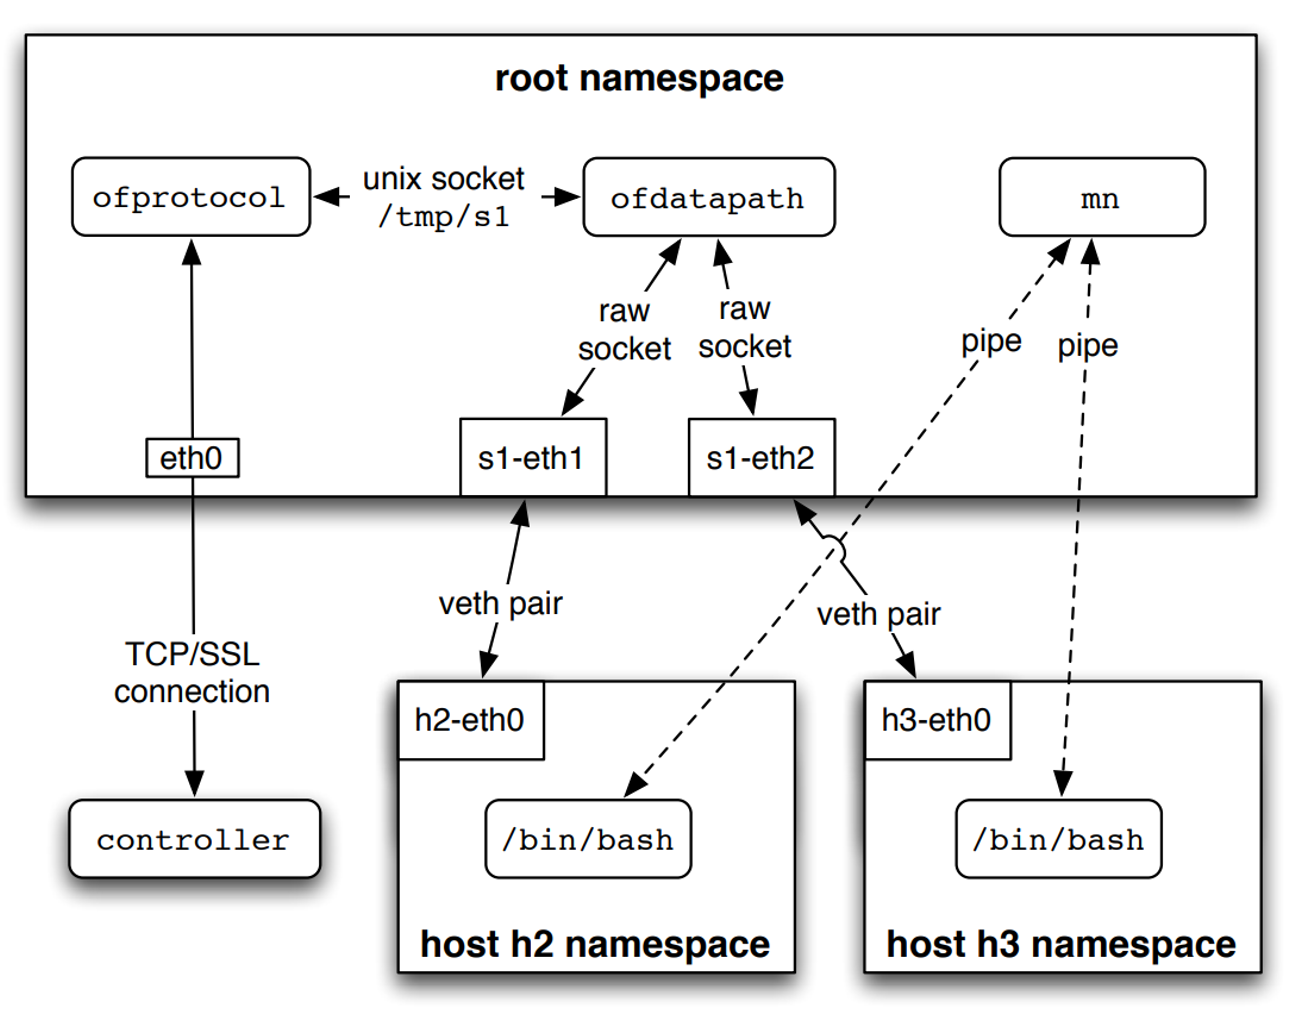
\includegraphics[width=11.5cm]{archivos/img/teoria/mn_arch.png}
    \caption{Arquitectura de Mininet \cite{heller2013reproducible}}
    \label{fig:mininet_arch}
\end{figure}

Una vez expuesta toda la teoría sobre Mininet, podría surgir la siguiente pregunta, ¿Cómo se puede comprobar que realmente hace uso de \textit{Network Namespaces}? Lo primero que se debe hacer es levantar el escenario para que así, Mininet cree las \textit{Network namespaces} que tenga que crear. En este caso, se utilizará la topología expuesta en la figura \ref{fig:mininet_arch}, para levantar dicha topología únicamente se tiene que tener Mininet instalado y seguir los pasos que se indican el bloque \ref{code:scenarioMininet}. 


 \begin{lstlisting}[language= bash, style=Consola, caption={Levantamiento de la topología de ejemplo},label=code:scenarioMininet]
    # Por defecto siempre carga la topología descrita en la figura anterior
    sudo mn
    
\end{lstlisting}
\vspace{0.5cm}

\begin{figure}[ht]
    \centering
    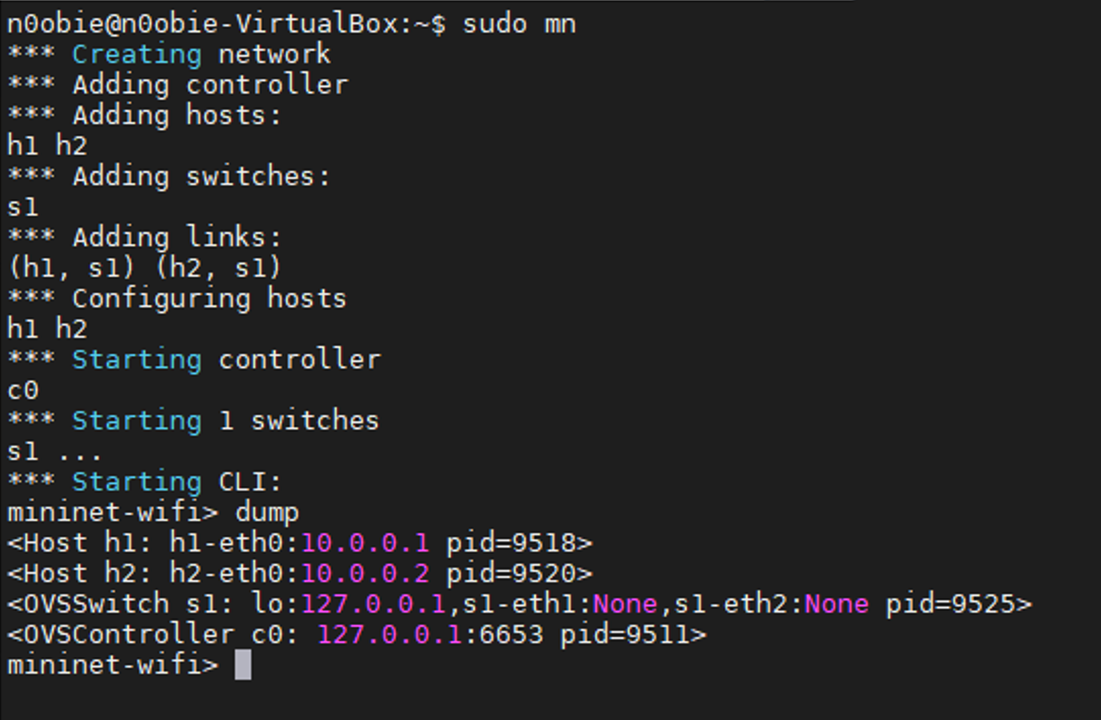
\includegraphics[width=9.5cm]{archivos/img/teoria/mn_01.png}
    \caption{Topología de ejemplo levantada}
    \label{fig:mininet_01}
\end{figure}

Ahora que ya se ha levantado el escenario se debería ser capaces de poder ver si hay \textit{Network Namespaces} en el sistema, para ello se hará uso del \textit{pack} de herramientas iproute2 (Ir a \ref{iproute2}). El comando por excelencia para listar las \textit{Network Namespaces} haciendo uso del módulo \textbf{netns} se puede ver en el bloque \ref{code:MininetNs}.


\begin{lstlisting}[language= bash, style=Consola, caption={Listar Network Namespaces},label=code:MininetNs]
    sudo ip netns list
\end{lstlisting}
\vspace{0.5cm}

\begin{figure}[ht]
    \centering
    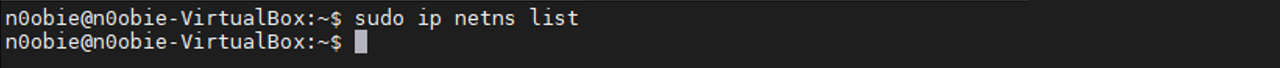
\includegraphics[width=15.5cm]{archivos/img/teoria/mn_02.png}
    \caption{Listado de Network Namespaces existentes en el sistema}
    \label{fig:mininet_02}
\end{figure}

Según se puede apreciar en la figura \ref{fig:mininet_02}, no parece que haya ninguna \textit{Network Namespace} en el sistema, pero entonces, ¿Dónde está el problema? El problema de que el comando \texttt{ip netns list} no arroje información, es que Mininet no está creando el \textit{softlink} requerido para que la herramienta sea capaz de listar las \textit{Network Namespaces}. Atendiendo a la documentación del comando se puede averiguar que dicho comando lee del path \texttt{/var/run/netns/} donde se encuentran todas las \textit{Network Namespaces} con nombre\footnote{Aquellas Netns las cuales se ha hecho un bindmount con su nombre en ese directorio para que persistan aunque no haya ningún proceso corriendo en ellas.}.\\
\par
Como ya se explicó, las \textit{Namespaces} tienen una vida finita, éstas viven siempre y cuando estén referenciadas (Ir a \ref{tab:linux_ns}), por tanto, si ninguna condición de referenciación se cumple, la \textit{Namespace} en cuestión es eliminada.\\
\par
Mininet se encarga de recrear la red emulada, y cuando el usuario termine la emulación, la red emulada debe desaparecer, este proceso debe ser lo más ligero y rápido posible para así ofrecer una mejor experiencia al usuario. La naturaleza del diseño de Mininet incita a pensar que la creación y destrucción de las \textit{Network Namespace} vienen asociadas a la primera condición de refereciación de una \textit{Namespace}. \\
\par
Es decir, no tendría sentido hacer \textit{mounts} ni \textit{softlinks} que a posteriori se deberán eliminar, ya que supondría una carga de trabajo bastante significativa para emulaciones de redes grandes y un aumento del tiempo destinado a la limpieza del sistema una vez que la emulación haya terminado. Además, se debe tener en cuenta que existe una condición que es bastante idónea con las necesidades de Mininet, ya que solo es necesario un proceso corriendo por cada \textit{Network Namespace}, y a la hora de limpiar únicamente se debe terminar con los procesos que sostienen las \textit{Network Namespace}. Cuando ya no haya ningún proceso corriendo en la \textit{Namespace}, y el Kernel se encargará de eliminar las \textit{Namespaces}.\\
\par
Según el razonamiento expuesto, se debería ver varios procesos que son creados a la hora del levantamiento del escenario en Mininet. Estos procesos deberán tener cada uno un fichero de \textit{Network Namespace}, \texttt{/proc/\{pid\}/ns/net}, con un \textit{inode} distinto para aquellos procesos que corren en distintas \textit{Network Namespaces}.\\

\begin{figure}[ht]
    \centering
    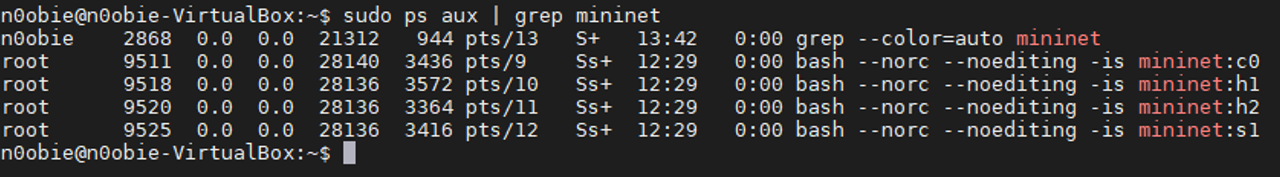
\includegraphics[width=15.5cm]{archivos/img/teoria/mn_03.png}
    \caption{Listado de procesos asociados a Mininet}
    \label{fig:mininet_03}
\end{figure}

Si se inspecciona el fichero \texttt{/proc/\{pid\}/ns/net} para cada proceso indicado en la figura \ref{fig:mininet_03} se podrá ver cuales de ellos están en una \textit{Network Namespace} distinta, en función del valor que tenga el \textit{inode}. Por ejemplo, se va a comprobar los procesos asociados a los \texttt{Host1} y \texttt{Host2}.\\
\par

\begin{figure}[ht]
    \centering
    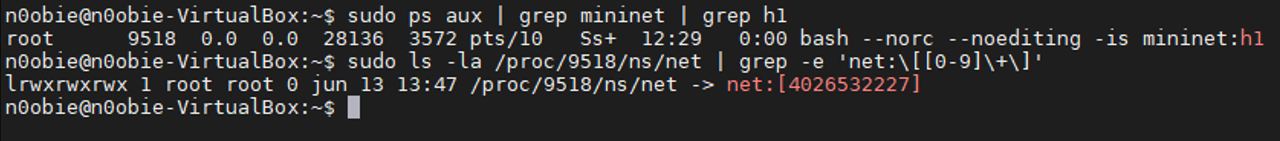
\includegraphics[width=15.5cm]{archivos/img/teoria/mn_04.png}
    \caption{Información relativa al proceso del Host1}
    \label{fig:mininet_04}
\end{figure}

\newpage

\begin{figure}[ht]
    \centering
    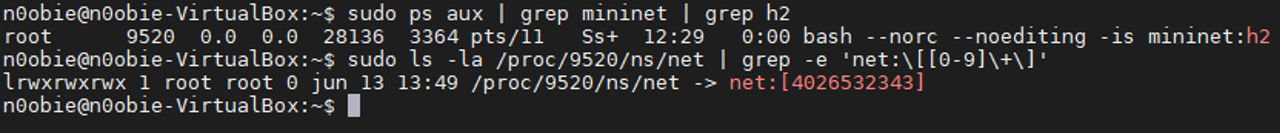
\includegraphics[width=15.5cm]{archivos/img/teoria/mn_05.png}
    \caption{Información relativa al proceso del Host2}
    \label{fig:mininet_05}
\end{figure}

Como se puede ver, \textit{inode} distintos, ficheros distintos, distintas \textit{Network namespaces}. Con esta prueba se puede ver como Mininet hace uso de procesos de bash para sostener las \textit{Network Namespaces} de los nodos que lo requieran. 

\subsection{Mininet CLI}

Mininet incluye una \gls{cli}, la cual puede ser invocada desde el script donde se describe la topología. Dicha \gls{cli}, contiene una gran variedad de comandos, por ejemplo listar la red, tirar enlaces, comprobar el estado de las interfaces, abrir una \textit{xterm} a un nodo, etc. A continuación se indica la tabla \ref{tab:cmdsMininet}, la cual resume todos los comandos existentes a día de hoy, para una explicación de cada uno de ellos en detalle se recomienda seguir esta \href{https://github.com/mininet/mininet/wiki/Introduction-to-Mininet}{\textbf{guía}}\footnote{\url{https://github.com/mininet/mininet/wiki/Introduction-to-Mininet}}.\\
\par

\begin{table}[!ht]
\centering
\begin{tabular}{|c|c|c|c|c|c|}
\hline
\texttt{EOF}      & \texttt{gterm}    & \texttt{links}   & \texttt{pingallfull}  & \texttt{py}     & \texttt{stop}   \\ \hline
\texttt{distance} & \texttt{help}     & \texttt{net}     & \texttt{pingpair}     & \texttt{quit}   & \texttt{switch} \\ \hline
\texttt{dpctl}    & \texttt{intfs}    & \texttt{nodes}   & \texttt{pingpairfull} & \texttt{sh}     & \texttt{time}   \\ \hline
\texttt{dump}     & \texttt{iperf}    & \texttt{noecho}  & \texttt{ports}        & \texttt{source} & \texttt{x}      \\ \hline
\texttt{exit}     & \texttt{iperfudp} & \texttt{pingall} & \texttt{px}           & \texttt{start}  & \texttt{xterm}  \\ \hline
\end{tabular}
\centering
\caption{Resumen comandos existentes en Mininet}
\label{tab:cmdsMininet}
\end{table}


\subsection{Mininet-WiFi}

Mininet-WiFi \cite{7367387} es un emulador de redes inalámbricas diseñado principalmente para trabajar bajo el estándar \texttt{ieee80211}. Esta herramienta nació de Mininet, es decir, es un \textit{fork} de la misma. Por ello, comparten todas las bases sobre virtualización ``ligera" haciendo uso de \textit{Namespaces} y \gls{veth}s, por tanto, todos los scripts de Mininet son compatibles en Mininet-WiFi. \\
\par
Esto es así ya que toda la funcionalidad wireless es un añadido sobre la base que desarrollaron para Mininet. Los desarrolladores de Mininet-WiFi se valieron del subsistema wireless del Kernel de Linux y del módulo mac80211\_hwsim, para conseguir emular las interfaces y el supuesto medio inalámbrico. Para más información sobre esta herramienta se recomienda ir al \textbf{punto} \ref{mn-wifi_bmv2_integration}, donde se hace un análisis profundo sobre las jerarquías de clases añadidas en Mininet-WiFi, como opera internamente y como se comunica con el módulo en el kernel para generar los escenarios inalámbricos.



\subsection{Mininet-IoT}
\label{mininetIoT}

La herramienta Mininet-IoT \cite{mininetIOT} es un emulador de redes de baja capacidad diseñado para trabajar en conjunto bajo el estándar \texttt{ieee802154} y la capa de adaptación 6LoWPAN. Esta herramienta nació de Mininet-WiFi, que a su vez nació de Mininet, por lo que en la práctica, Mininet-IoT comparte todas las técnicas de virtualización ``ligera" de Mininet. Al heredar de Mininet-WiFi y Mininet, todos los scripts para desplegar topologías alámbricas y WiFi son compatibles en Mininet-IoT.  \\
\par

La gran diferencia entre Mininet-IoT y Mininet-WiFi, radica en el módulo que emplean para conseguir emular las interfaces y el supuesto medio inalámbrico. Mininet-WiFi hace uso del módulo mac80211\_hwsim, mientras que Mininet-IoT hace uso del módulo del Kernel mac802154\_hwsim (es necesario tener una versión del Kernel superior a la \texttt{4.18.x} para obtener dicho modulo). Toda la gestión de nodos, interfaces y enlaces es exactamente la misma a la de Mininet-WiFi. Por ello, Ramon Fontes (principal desarrollador de la herramienta), creó una clase agnóstica para gestionar módulos del Kernel en Mininet-WiFi, y migró todo el proyecto de Mininet-IoT a Mininet-WiFi. De esta forma, el mantenimiento del \textit{core} que compartían ambas herramientas se hacía únicamente en un proyecto, y daba la posibilidad al usuario de Mininet-WiFi de establecer enlaces de baja capacidad en sus topologías inalámbricas.  